\chapter{Arhitektura i dizajn sustava}
			
		\text Arhitektura se može podijeliti na tri podsustava:
		\begin{packed_item}
			
			\item Web poslužitelj
			\item Web aplikacija
			\item Baza podataka
			
		\end{packed_item}

		\begin{figure}[H]
			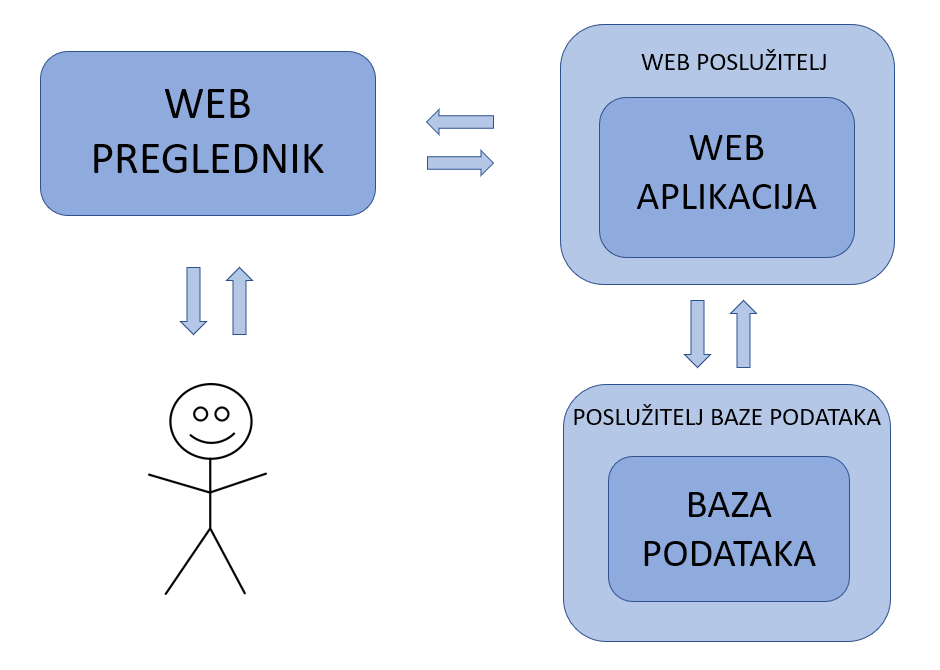
\includegraphics[scale=0.50]{slike/arhitektura.png} %veličina slike u odnosu na originalnu datoteku i pozicija slike
			\centering
			\caption{Arhitektura sustava}
			\label{fig:arhitekura slika}
		\end{figure}
	
		\textit {\underbar {Web preglednik}} \text je program koji služi za pregledavanje web-stranica. Uloga web preglednika je da kada korisnik zatraži određenu stranicu dohvati potreban sadržaj s web poslužitelja i prikaže ga korisniku. 
		
		\textit {\underbar {Web poslužitelj}} \text omogućuju komunikaciju klijenta s aplikacijom tako da proslijedi zahtjev klijenta aplikaciji i odgovor kojeg je stvorila aplikacija natrag klijentu. Komunikacija se odvija preko HTTP-a, internetskog protokola aplikacijskog sloja koji služi za prijenos dokumenata poput onih pisanih u HTML-u. 
		
		\textit {\underbar {Web aplikacija}} \text omogućuje klijentu postavljanje zahtjeva na koje ona stvara odgovore. Ovisno o zahtjevu može pristupati bazi podataka te onda generira odgovor kojeg šalje u obliku HTML dokumenta pregledniku kojeg koristi klijent.
		
		\textit {\underbar {Poslužitelj baze podataka}} \text omogućuje web aplikaciji  dohvaćanje sadržaja iz baze podataka i zapisivanje novih stavki u bazu podataka.
		
		\text Za izradu frontenda korišten je programski jezik JavaScript i radni okvir React. React je JavaScript biblioteka koja služi za izradu korisničkih sučelja. Za izradu backenda korišten je programski jezik Java i radni okvir Spring Boot koji omogućuje brži i efikasniji razvoj aplikacije. Korišteno razvojno okruženje je Microsoft Visual Studio. Arhitektura sustava temeljiti će se na MVC (Model-View-Controller) konceptu.
		
		Svrha MVC obrasca je odvajanje programske logike u tri međusobno povezana dijela, čime se poštuje načelo odvajanja briga i olakšava razvoj aplikacije.
		
		\begin{figure}[H]
			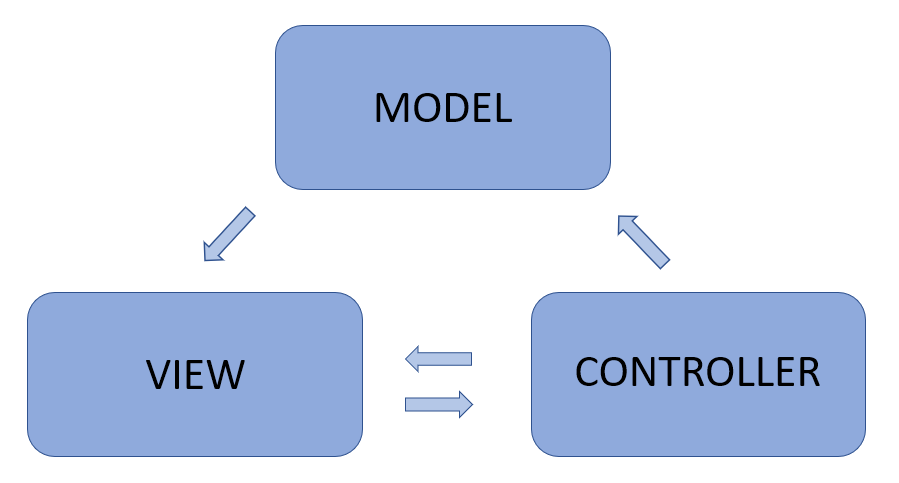
\includegraphics[scale=0.50]{slike/mvc.png} %veličina slike u odnosu na originalnu datoteku i pozicija slike
			\centering
			\caption{MVC dijagram}
			\label{fig:mvc model}
		\end{figure}
	
		\text MVC se sastoji od:
		\begin{packed_item}
			
			\item Model - centralna komponenta koja upravlja podacima, logikom i pravilima aplikacije
			\item View - prikazuje podatke modela i šalje radnje korisnika kontroleru
			\item Controller - prima radnje korisnika na temelju kojih vrši daljnu interakciju s modelom i pogledom
			
		\end{packed_item}

				
		\section{Baza podataka}
			
		\text Za potrebe našeg sustava koristit ćemo relacijsku bazu podataka koja svojom strukturom olakšava modeliranje stvarnog svijeta. Gradivna jedinka baze je relacija, odnosno tablica koja je definirana svojim imenom i skupom atributa. Zadaća baze podataka je brza i jednostavna pohrana, izmjena i dohvat podataka za daljnju obradu.
		\text Baza podataka se sastoji od idućih entiteta:
		\begin{packed_item}
			
			\item User
			\item Responder
			\item Station
			\item Call
			\item CallRequest
			\item Photo
			\item Task
			\item CallComments

		\end{packed_item}
		
			\subsection{Opis tablica}

				\textbf {User} \text Ovaj entitet sadrži općenite informacije o svim korisnicima aplikacije. Sadrži atribute: Username, PhotoURL, PasswordHash, Name, Surname, PhoneNumber, eMail, Role i Confirmed. Ovaj entitet je u vezi \textit{One-to-one} s entitetom Responder preko atributa Username, u vezi \textit{One-to-many} s entitetom CallRequest preko atributa DispatcherUsername te je u vezi \textit{One-to-many} s entitetom Task preko atributa DispatcherUsername. 
				
				
				\begin{longtblr}[
					label=none,
					entry=none
					]{
						width = \textwidth,
						colspec={|X[6,l]|X[6, l]|X[20, l]|}, 
						rowhead = 1,
					} %definicija širine tablice, širine stupaca, poravnanje i broja redaka naslova tablice
					\hline \multicolumn{3}{|c|}{\textbf{Username}}	 \\ \hline[3pt]
					\SetCell{LightGreen}Username & VARCHAR & jedinstveno korisničko ime  	 	\\ \hline
					PhotoURL & VARCHAR & url fotografije	\\ \hline
					PasswordHash	& VARCHAR & hash lozinke 	\\ \hline
					Name & VARCHAR & Ime korisnika  	\\ \hline
					Surname & VARCHAR & Prezime korisnika  	\\ \hline
					eMail & VARCHAR & e-mail korisnika  \\ \hline 
					PhoneNumber & VARCHAR & Broj mobitela korisnika  	\\ \hline 
					Role & VARCHAR	& Uloga korisnika		\\ \hline
					Confirmed & BIT & Status registracije korisnika \\ \hline   
				\end{longtblr}



				\textbf {Responder} \text Ovaj entitet sadrži sve važne informacije o spasiocima. Sadrži atribute: Username, Qualification, LocationLatitude, LocationLongitude, Availability, CallName i StationName. Ovaj entitet je u vezi \textit{One-to-one} sa entitetom User preko atributa Username, u vezi \textit{One-to-many} sa entitetom CallRequest preko atributa ResponderUsername, u vezi \textit{One-to-one} s entitetom Station preko atributa StationName, u vezi \textit{One-to-one} s entitetom Station preko atributa StationChief, u vezi \textit{One-to-Many} s entitetom Task preko atributa ResponderUsername, u vezi \textit{One-to-Many} s entitetom CallComents preko atributa Username te u vezi \textit{One-to-one} s entitetom Call preko atributa CallName.
				
				
				\begin{longtblr}[
					label=none,
					entry=none
					]{
						width = \textwidth,
						colspec={|X[8,l]|X[6, l]|X[20, l]|}, 
						rowhead = 1,
					} %definicija širine tablice, širine stupaca, poravnanje i broja redaka naslova tablice
					\hline \multicolumn{3}{|c|}{\textbf{Responder}}	 \\ \hline[3pt]
					\SetCell{LightGreen}Username & VARCHAR	&  	Korisničko ime spasioca  	\\ \hline
					Qualification	& VARCHAR &  Osposobljenje spasioca 	\\ \hline 
					Location Latitutude & VARCHAR &  Geografska širina lokacije spasioca \\ \hline 
					Location Longitude & VARCHAR & Geografska dužina lokacije spasioca \\ \hline 
					Availability & BIT	&  Status zauzetosti spasioca 		\\ \hline 
					\SetCell{LightBlue} CallName	& VARCHAR & Ime akcije u kojoj spasilac trenutno sudjeluje \\ \hline 
					\SetCell{LightBlue} StationName	& VARCHAR &  Ime stanice kojoj spasilac pripada \\ \hline 
				\end{longtblr}
			
				

				\textbf{Call} \text Ovaj entitet sadrži sve važne informacije o akciji. Sadrži atribute: CallName, Address, Finished i Description. Ovaj entitet je u 						             vezi \textit{One-to-one} s entitetom Responder preko atributa CallName, u vezi \textit{One-to-many} s entitetom Photo preko atributa CallName, u vezi \textit{One-to-many} s entitetom CallComments preko atributa CallName te u 									     vezi \textit{One-to-many} s entitetom CallRequest preko atributa CallName.
				
				
				\begin{longtblr}[
					label=none,
					entry=none
					]{
						width = \textwidth,
						colspec={|X[6,l]|X[6, l]|X[20, l]|}, 
						rowhead = 1,
					} %definicija širine tablice, širine stupaca, poravnanje i broja redaka naslova tablice
					\hline \multicolumn{3}{|c|}{\textbf{Call}}	 \\ \hline[3pt]
					\SetCell{LightGreen}CallName & VARCHAR	&  	Ime akcije  	\\ \hline
					Address	& VARCHAR &  Adresa  	\\ \hline 
					Finished & BIT &  Oznaka završetka akcije \\ \hline 
					Description & VARCHAR	&  Kratak opis akcije		\\ \hline 
				\end{longtblr}

				
				\textbf{CallRequest} \text Ovaj entitet sadrži sve važne informacije o pozivu na akciju pojedinačnom spasiocu. Sadrži atribute: CallName, ResponderUsername, DispatcherUsername, ResponderResponse, ResponderRole, Urgency i Comment. Ovaj entitet je u vezi \textit{Many-to-one} s entitetom Responder preko atributa ResponderUsername, u vezi \textit{Many-to-many} s entitetom User preko atributa DispatcherUsername te u vezi \textit{Many-to-one} s entitetom Call preko atributa CallName.
				
				
				\begin{longtblr}[
					label=none,
					entry=none
					]{
						width = \textwidth,
						colspec={|X[8,l]|X[6, l]|X[20, l]|}, 
						rowhead = 1,
					} %definicija širine tablice, širine stupaca, poravnanje i broja redaka naslova tablice
					\hline \multicolumn{3}{|c|}{\textbf{CallRequest}}	 \\ \hline[3pt]
					\SetCell{LightGreen}CallName & VARCHAR	&  	Ime akcije za koju se šalje poziv  	\\ \hline
					\SetCell{LightGreen}Respoder Username & VARCHAR	&  	Korisničko ime spasioca kojem je poslan poziv  	\\ \hline  
					\SetCell{LightBlue} Dispatcher Username	& VARCHAR &   	Korisničko ime dispečera koji je poslao poziv\\ \hline 
					Responder Response & BIT	&  Prihvat poziva ili odbijanje\\ \hline
					Responder Role	& VARCHAR & Način sudjelovanja spasioca  	\\ \hline 
					Urgency & INT & Razina hitnosti  \\ \hline 
					Comment	& VARCHAR & Komentar dispečera  	\\ \hline
				\end{longtblr}
				
				\textbf{Task} \text Ovaj entitet sadrži sve važne informacije o zadatku kojeg dispečer zadaje spasiocima. Sadrži atribute: IDTask, Comment, Description, Address, ResponderUsername i DispatcherUsername. Ovaj entitet je u vezi \textit{Many-to-one} s entitetom User preko atributa DispatcherUsername te u vezi \textit{Many-to-one} s entitetom Responder preko atributa ResponderUsername.
				
				
				\begin{longtblr}[
					label=none,
					entry=none
					]{
						width = \textwidth,
						colspec={|X[6,l]|X[6, l]|X[20, l]|}, 
						rowhead = 1,
					} %definicija širine tablice, širine stupaca, poravnanje i broja redaka naslova tablice
					\hline \multicolumn{3}{|c|}{\textbf{Task}}	 \\ \hline[3pt]
					\SetCell{LightGreen}IDTask & INT & Identifikator zadatka	\\ \hline 		
					Comment	& VARCHAR & Komentar kojeg može dati dispečer  	\\ \hline
					Description & VARCHAR & Opis zadatka  \\ \hline
					Address	& VARCHAR & Adresa na koju treba doći\\ \hline
					\SetCell{LightBlue} Responder Username	& VARCHAR &   	Korisničko ime spasioca koji je dobio zadatak\\ \hline 
					\SetCell{LightBlue} Dispatcher Username	& VARCHAR &   	Korisničko ime dispečera koji je zadao zadatak\\ \hline 
				\end{longtblr}
			
				\textbf{Photo} \text Ovaj entitet sadrži fotografije akcija. Sadrži atribute: PhotoURL i CallName. Ovaj entitet je u vezi \textit{Many-to-one} s entitetom Call preko atributa CallName.
				
				
				\begin{longtblr}[
					label=none,
					entry=none
					]{
						width = \textwidth,
						colspec={|X[6,l]|X[6, l]|X[20, l]|}, 
						rowhead = 1,
					} %definicija širine tablice, širine stupaca, poravnanje i broja redaka naslova tablice
					\hline \multicolumn{3}{|c|}{\textbf{Photo}}	 \\ \hline[3pt]
					\SetCell{LightGreen}PhotoURL & VARCHAR	&  Url fotografije akcije  	\\ \hline
					\SetCell{LightBlue} CallName	& VARCHAR & Ime akcije kojoj fotografija pripada  	\\ \hline 
				\end{longtblr}
			
				\textbf{CallComments} \text Ovaj entitet sadrži sve važne informacije vezane uz mogućnost spasilaca da komentiraju akcije. Sadrži atribute: CallName, Username, Comment, Locationlatitude i LocationLongitude. Ovaj entitet je u vezi \textit{Many-to-one} s entitetom Call preko atributa CallName te u vezi \textit{Many-to-one} s entitetom Responder preko atributa Username.
				
				
				\begin{longtblr}[
					label=none,
					entry=none
					]{
						width = \textwidth,
						colspec={|X[8,l]|X[6, l]|X[20, l]|}, 
						rowhead = 1,
					} %definicija širine tablice, širine stupaca, poravnanje i broja redaka naslova tablice
					\hline \multicolumn{3}{|c|}{\textbf{CallComments}}	 \\ \hline[3pt]
					\SetCell{LightGreen}CallName & VARCHAR	&  Ime akcije za koju se ostavlja komentar  	\\ \hline
					\SetCell{LightGreen} Username	& VARCHAR & Korisnik koji ostavlja komentar \\ \hline 
					Comment	& VARCHAR & Komentar kojeg je korisnik ostavio  	\\ \hline 
					Location Latitude & VARCHAR &  Geografska širina lokacije komentara \\ \hline 
					Location Longitude & VARCHAR & Geografska dužina lokacije komentara \\ \hline 
				\end{longtblr}
			
				\textbf{Station} \text Ovaj entitet sadrži sve važne informacije vezane uz stanicu. Sadrži atribute: StationName i StationChief. Ovaj entitet je u vezi \textit{One-to-one} s entitetom Responder preko atributa StationName te u vezi \textit{One-to-one} s entitetom Responder preko atributa StationChief.
				
				
				\begin{longtblr}[
					label=none,
					entry=none
					]{
						width = \textwidth,
						colspec={|X[6,l]|X[6, l]|X[20, l]|}, 
						rowhead = 1,
					} %definicija širine tablice, širine stupaca, poravnanje i broja redaka naslova tablice
					\hline \multicolumn{3}{|c|}{\textbf{Station}}	 \\ \hline[3pt]
					\SetCell{LightGreen}StationName	& VARCHAR & Naziv stanice \\ \hline 
					\SetCell{LightBlue}StationChief	& VARCHAR & Korisničko ime voditelja stanice\\ \hline 
				\end{longtblr}
				

				
			
			\subsection{Dijagram baze podataka}
				

				\begin{figure}[H]
					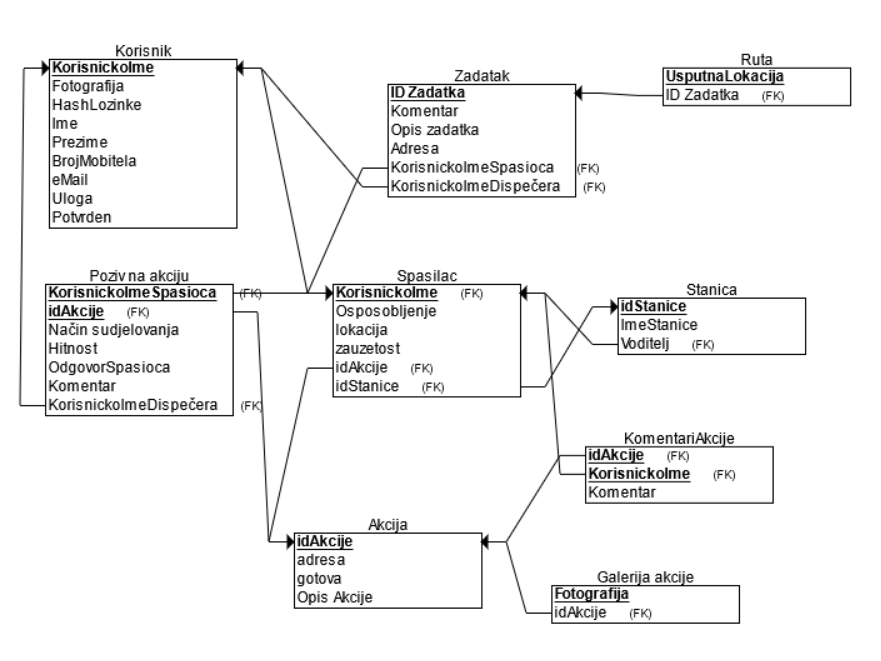
\includegraphics[scale=0.40]{slike/ModelBazePodataka.png} %veličina slike u odnosu na originalnu datoteku i pozicija slike
					\centering
					\caption{Dijagram baze podataka}
					\label{fig:baza podataka}
				\end{figure}
			
			\eject
			
			
		\section{Dijagram razreda}
		
			\begin{figure}[H]
				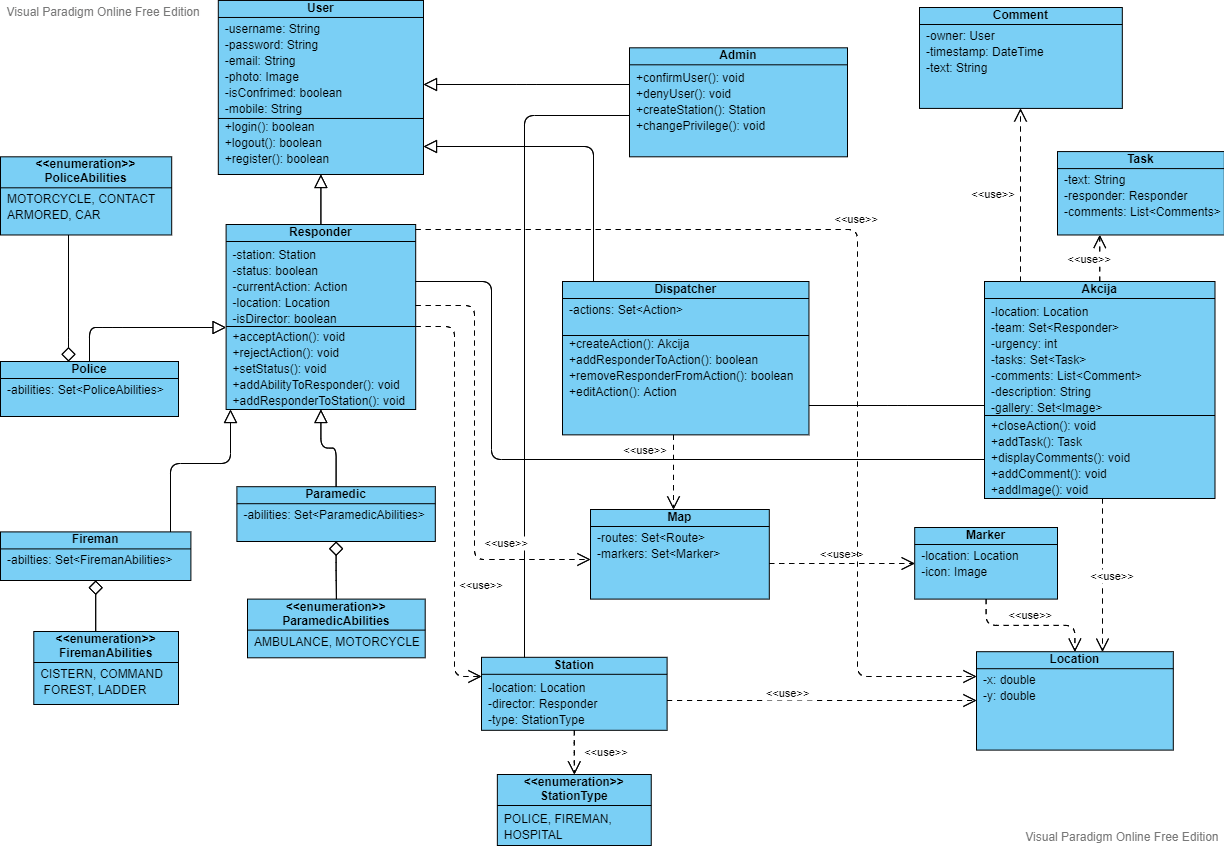
\includegraphics[scale=0.4]{slike/classes.PNG}
				\centering
				\caption{Dijagram razreda}
				\label{fig:razredi}
			\end{figure}
			
			\textbf{\textit{dio 2. revizije}}\\			
			
			\textit{Prilikom druge predaje projekta dijagram razreda i opisi moraju odgovarati stvarnom stanju implementacije}
			
			
			
			\eject
		
		\section{Dijagram stanja}
			
			
			\textbf{\textit{dio 2. revizije}}\\
			
			\textit{Potrebno je priložiti dijagram stanja i opisati ga. Dovoljan je jedan dijagram stanja koji prikazuje \textbf{značajan dio funkcionalnosti} sustava. Na primjer, stanja korisničkog sučelja i tijek korištenja neke ključne funkcionalnosti jesu značajan dio sustava, a registracija i prijava nisu. }
			
			
			\eject 
		
		\section{Dijagram aktivnosti}
			
			\begin{figure}[H]
				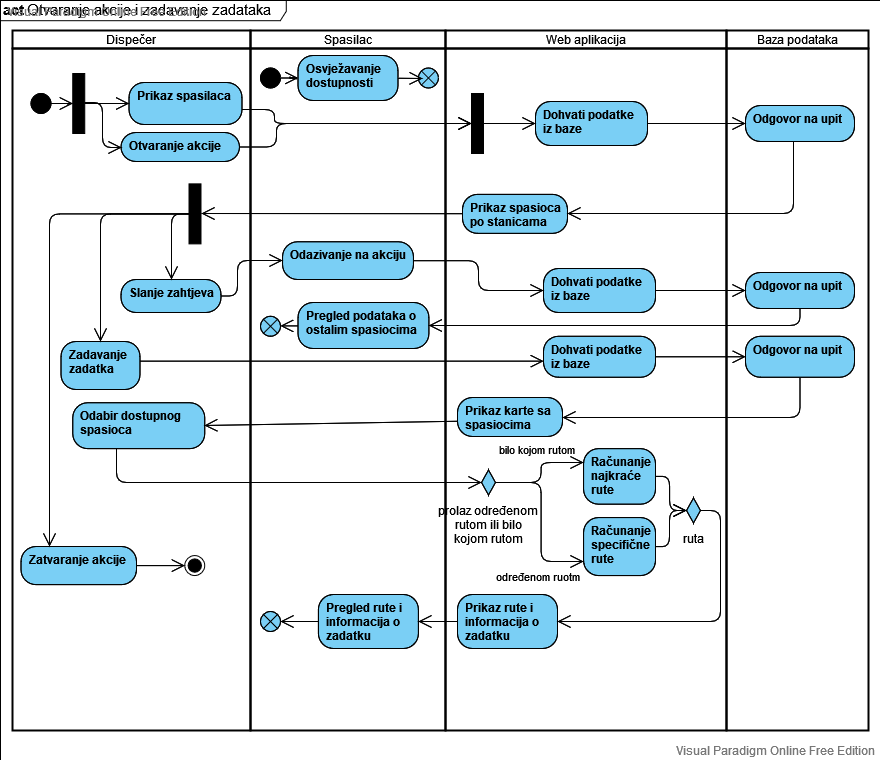
\includegraphics[scale=0.5]{slike/act.png}
				\centering
				\caption{Dijagram aktivnosti}
				\label{fig:act}
			\end{figure}
			Prikaz akcije otvaranja akcije za spasioce i zadavanja zadatka. Dispečer otvara i zatvara akcije, te zadaje zadatke. Spasioc osvježava svoju dostupnost i odaziva se na akcije. Dispečeru se prikazuju spasioci po stanicama i na karti. Spasiocu se prikazuju informacije o zadatku i ostalim spasiocima.
			\eject
			
		\section{Dijagram komponenti}
		
			\begin{figure}[H]
				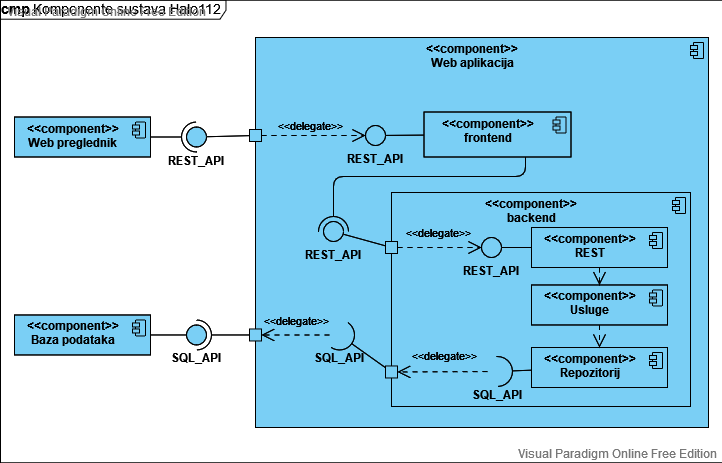
\includegraphics[scale=0.6]{slike/cmp.png}
				\centering
				\caption{Dijagram komponenti}
				\label{fig:cmp}
			\end{figure}
			Prikaz komponenti i strukture čitavog sustava. Korinik komunicira sa sustavom pomoću HTTP zahtjeva. Frontend i backend također komuniciraju HTTP porukama. Razmjenu HTTP poruka omogućuje REST API. Backend se sastoji od tri sloja. REST nadglednici komuniciraju s frontendom, a JPA repozitorij pohranjuje entitete sustava u bazu podataka korištenjem SQL API-a. Na sloju usluge je ostvarena temeljna funkcionalnost.